\documentclass{beamer}
\usepackage[utf8]{inputenc}
\usepackage{amsmath, amssymb}
\usepackage{bbm}
\usepackage{dsfont}

\usetheme{Madrid}
\setbeamerfont{normal text}{size=\small}

\title{Estimation and Inference of Causal Effects for \\ Spatially Clustered Survival Data: A Non-parametric \\ Bayesian Approach}
\author{Durbadal Ghosh}
\date{\today}

%%%%%%%%%%%%%%%%%%%%%%%%%%%%%%%%%%%%%%%%%%%%%%%%%%%%%%%%%%%%%%
\begin{document}

%%%%%%%%%%%%%%%%%%%%%%%%%%%%%%%%%%%%%%%%%%%%%%%%%%%%%%%%%%%%%%
\begin{frame}
  \titlepage
\end{frame}

%%%%%%%%%%%%%%%%%%%%%%%%%%%%%%%%%%%%%%%%%%%%%%%%%%%%%%%%%%%%%%


\section{Motivation}



\begin{frame}{Florida Cancer Registry}
    \begin{itemize}
      \vfill \item \textbf{Data:}
      \begin{itemize}
        \vfill \item 76,106 breast cancer patients from 67 counties in FL
        \vfill \item Spatial clustering by county
        \vfill \item Time-to-death (right-censored)
        \vfill \item Treatment: delay ($>$90 days) vs no delay
      \end{itemize}
      \vspace{6pt}
      \vfill \item \textbf{Goal:}
      \begin{itemize}
        \vfill \item Estimate average and county-level causal effects
        \vfill \item Adjust for patient and county-level confounders
        \vfill \item Address spatial clustering
      \end{itemize}
      \vspace{6pt}
      \vfill \item \textbf{Our Approach:}
      \begin{itemize}
        \vfill \item Bayesian non-parametric model using BART
        \vfill \item Handles spatial clustering, censoring, and confounding
      \end{itemize}
    \end{itemize}
    \end{frame}

%% Insert new frame after Florida Cancer Registry and before Why Two-Stage Method
\begin{frame}{Clustering, Spatial Effects, and BART in Causal Inference}
    \begin{itemize}
      \vfill \item \textbf{Why Account for Clustering and Spatial association?}
      \begin{itemize}
        \vfill \item Cluster members share hidden traits.
        \vfill \item Ignoring structure risks biased inference.
        \vfill \item Nearby units face similar environments.
        \vfill \item County-specific treatment effects are crucial.
      \end{itemize}
      \vspace{6pt}
      \vfill \item \textbf{Why BART?}
      \begin{itemize}
        \vfill \item Captures complex, nonlinear effects.
        \vfill \item Provides  uncertainty quantification
        \vfill \item Promising in causal settings.
      \end{itemize}
    \end{itemize}
    \end{frame}


\begin{frame}{Our Contributions}
    \begin{itemize}
      \vfill \item \textbf{Novel Integration:}
      \begin{itemize}
        \vfill \item Combines BART with spatial random effects
        \vfill \item Tailored for censored and clustered survival data
      \end{itemize}
      \vspace{6pt}
      \vfill \item \textbf{Methodological Advantages:}
      \begin{itemize}
        \vfill \item Complex treatment–outcome patterns in presence of confounding
        \vfill \item Spatial correlation via CAR priors

        \vfill \item Doubly robust two-stage procedure
        \vfill \item Full posterior for County-specific effects
      \end{itemize}
    \end{itemize}
    \end{frame}


\section{Methods}

\begin{frame}{Notation and Definitions}
  \begin{itemize}
    \vfill \item \(i = 1,\dots,K\): clusters; \(j = 1,\dots,n_i\): subjects; \(N = \sum_i n_i\)
    \vfill \item Treatment: \(z_{ij} \in \{0,1\}\)
    \vfill \item Confounders: \(\mathbf{x}_{ij}\) (individual), \(\mathbf{v}_i\) (cluster-level)
    \vfill \item Survival time: \(T_{ij}\), censoring time: \(C_{ij}\)
    \vfill \item Observed: \(y_{ij} = \min(T_{ij}, C_{ij})\), \(\delta_{ij} = \mathds{1}(T_{ij} < C_{ij})\)
    \vfill \item Counterfactuals: \(T_{ij}(1), T_{ij}(0)\), \(C_{ij}(1), C_{ij}(0)\)
  \end{itemize}
\end{frame}



\begin{frame}{Causal Estimands}
\begin{itemize}
  \vfill \item \textbf{Counterfactual Survival Functions:}
\begin{itemize}
    \vfill \item \( S^{(z)}(t \mid \mathbf{x}, \mathbf{v}) = P(T(z) \ge t \mid \mathbf{x}, \mathbf{v}) \)
    \vfill \item \( S^{(z)}(t) = \mathbb{E}_{\mathbf{x}, \mathbf{v}}[S^{(z)}(t \mid \mathbf{x}, \mathbf{v})] \)
  \end{itemize}
  \vspace{6pt}
  \vfill \item \textbf{Conditional Estimands:}
  \begin{itemize}
   \vfill \item \( \Delta^{\text{CATE}}(\mathbf{x}, \mathbf{v}) = \mathbb{E}[T(1) - T(0) \mid \mathbf{x}, \mathbf{v}] \)
    \vfill \item \( \Delta^{\text{CRATE}}(t,\mathbf{x}, \mathbf{v}) = \mathbb{E}[T(1) \wedge t - T(0) \wedge t \mid \mathbf{x}, \mathbf{v}] \)
    \end{itemize}
    \vspace{6pt}
  \vfill \item \textbf{Marginal Estimands:}
  \begin{itemize}
    \vfill \item  \( \Delta^{\text{SPTE}}(t) = S^{(1)}(t) - S^{(0)}(t) \)
    \vfill \item  \( \Delta^{\text{ATE}} = \mathbb{E}_{\mathbf{x},\mathbf{v}}[T(1)] - \mathbb{E}[T(0)] \)
    \vfill \item  \( \Delta^{\text{RATE}}(t) = \mathbb{E}_{\mathbf{x}, \mathbf{v}}[T(1) \wedge t - T(0) \wedge t] \)
\end{itemize}
\end{itemize}
\end{frame}
\begin{frame}{Causal Assumptions}
    \item \textbf{(A1) SUTVA:} For any two subjects \( j, j' \) in clusters \( i, i' \),
    \[
    T_{ij}(z_{ij}, z_{i'j'}) = T_{ij}(z_{ij})
    \]
    \item \textbf{(A2) Consistency:}
    \[
    T_{ij} = T_{ij}(1)\mathds{1}(Z_{ij}=1) + T_{ij}(0)\mathds{1}(Z_{ij}=0)
    \]
    \item \textbf{(A3) Unconfoundedness:}
    \[
    T_{ij}(z) \perp\!\!\!\perp Z_{ij} \mid \mathbf{x}_{ij}, \mathbf{v}_i, \quad z=0,1
    \]
    \item \textbf{(A4) Positivity:}
    \[
   e_{ij}= e(\mathbf{x}_{ij}, \mathbf{v}_i) = P(Z_{ij}=1 \mid \mathbf{x}_{ij}, \mathbf{v}_i)
    \]
    is bounded away from 0 and 1.
    \item \textbf{(A5) Covariate-dependent Censoring:}
    \[
    T_{ij}(z) \perp\!\!\!\perp C_{ij}(z) \mid \mathbf{x}_{ij}, \mathbf{v}_i, Z_{ij}=z, \quad z=0,1
    \]
\end{frame} 

\begin{frame}{Model for Propensity Score}
   
  $P[Z_{ij}=1\mid \mathbf{x}_{ij},\mathbf{v_i}]=e_{ij}$ (Propensity score) \\
  
  \\
  \textbf{Two-stage implementation:} \\
  \begin{enumerate}
    \vfill \item Estimate PS $\hat{e}_{ij}$
    \vfill \item Plug in $\hat{e}_{ij}$ into the survival model. (Doubly Robust)
  \end{enumerate}
  \vspace{6pt}

  \begin{itemize}
    \vfill \item \textbf{Advantages of Two-Stage Approach:}
    \begin{itemize}
        \vfill \item Issue with selection bias: $\Delta(z)=E[T(z)\mid Z=z]-E[T(z)]$
       \vfill \item Provides double robustness: consistent if either model is correctly specified
        \vfill \item Avoids feedback between treatment and outcome models
        \vfill \item Computationally efficient: separate estimation of PS and outcome models
    \end{itemize}
  \end{itemize}
  \vspace{6pt}
  \textbf{Model for Propensity Score:}\\
  $e_{ij}=\Phi(b_1(\mathbf{x}_{ij},\mathbf{v}_i)),$ where $b_1(\cdot)\sim BART$
  
\end{frame}

\begin{frame}{Bayesian Additive Regression Trees (BART)}
   
    \begin{itemize}
   
    \vfill \item
      \(b(\mathbf{x}) = \sum_{j=1}^{J}g(\mathbf{x} ; \tau_j, \mathcal{M}_j)\)
   \\
    \vspace{6pt}
        \(\tau_j\) : topology and splitting rules of tree \(k\)
  \\  \vspace{6pt} 
        \(\mathcal{M}_j = (\mu_{j1}, \dots, \mu_{jm_j})\): the set of predictions associated with the \(m_j\) terminal nodes of the tree \(j\) 
    \end{itemize}
   
    
    
    \begin{center}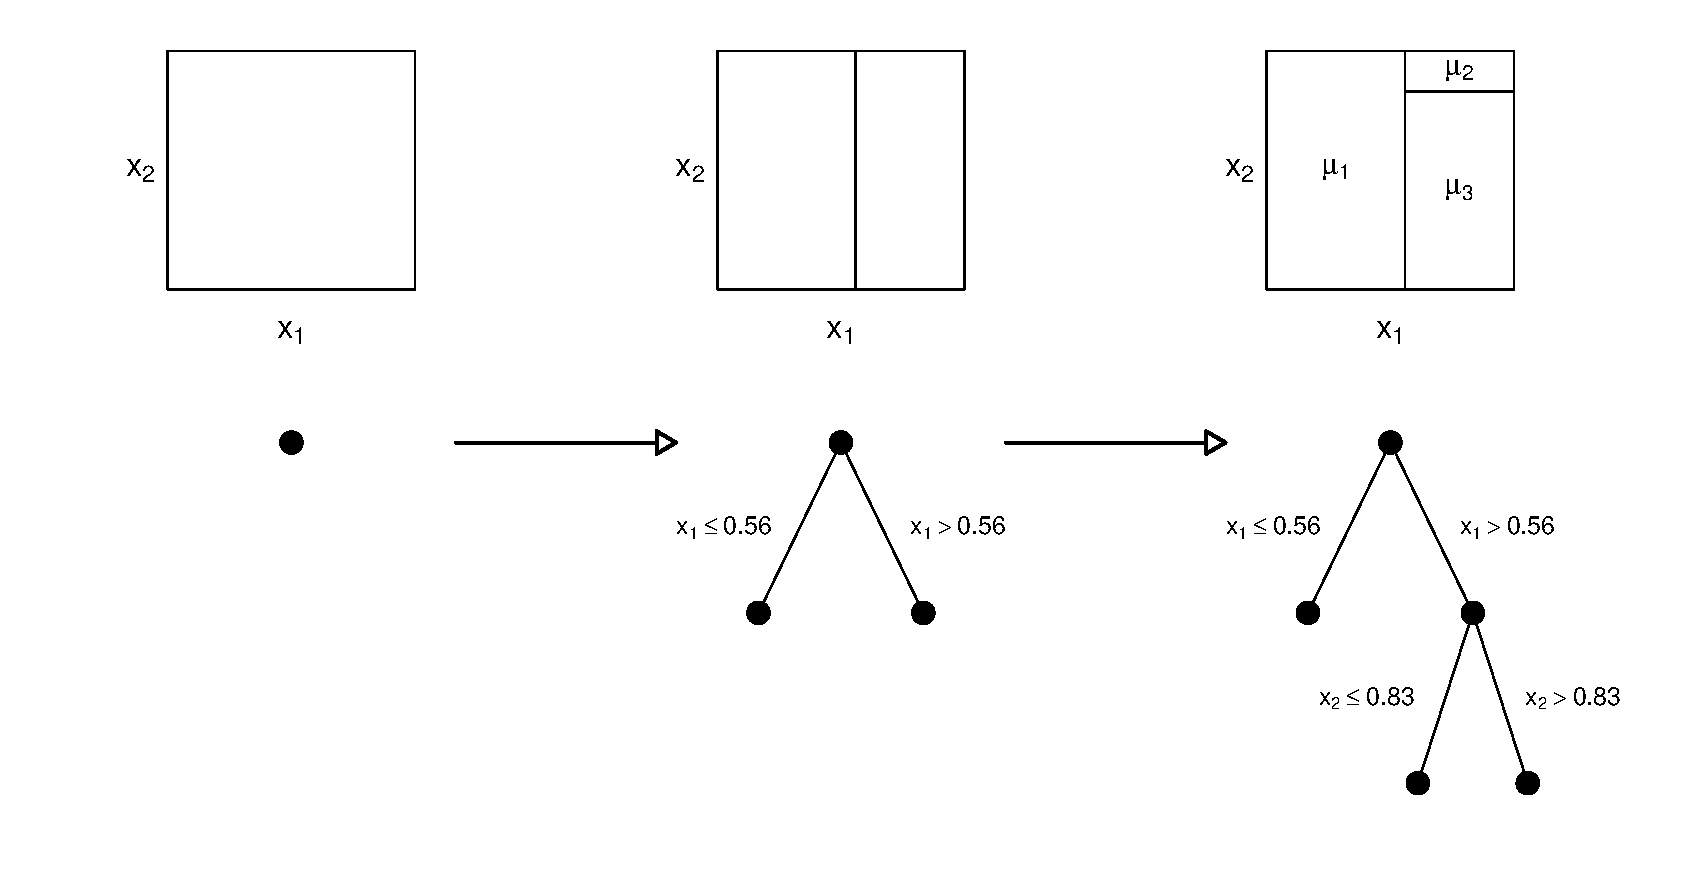
\includegraphics[width=.6\textwidth]{pics/BARTdiagram.eps} \end{center}
   \alert{SoftBART: Adds smoothness to BART}
\end{frame}
\begin{frame}{The Outcome Model}
  \begin{itemize}
    \vfill \item \textbf{Model:} 
      \[
      \log T_{ij} = b_2\Bigl(z_{ij},\mathbf{x}_{ij},\mathbf{v}_i,\hat{e}_{ij}\Bigr) + W_i + \epsilon_{ij},\quad \epsilon_{ij}\sim N(0,\sigma^2).
      \]
      
    \vfill \item \textbf{BART:} 
      \[
      b_2(\cdot) \sim SoftBART
      \]
      
      \vfill \item \textbf{Spatial Effects:} CAR prior on \(\mathbf{W}\): 
      \[
      p(\mathbf{W}) \propto \exp\left(-\frac{1}{2\sigma_\mathbf{W}^2} \mathbf{W}^\top (D - \rho A) \mathbf{W}\right)
      \]
      
      \vfill \item \textbf{Censoring:} Truncated normal latent variables .
\end{itemize}
\end{frame}
\section{Simulation}

\begin{frame}{Simulation Setup}
  \begin{itemize}
    \vfill \item \(n = 3000\) subjects, \(K = 15\) clusters (variable sizes)
    \vfill \item Confounders: \(X_1, X_2 \sim U(0,1)\)
    \vfill \item Propensity score:
    \[
    e = \text{expit}(0.3X_1 - 0.2X_2 + 0.5X_1X_2)
    \]
    \vfill \item Treatment: \(Z \sim \text{Bernoulli}(e)\)
    \vfill \item Censoring: \(C \sim \text{Exp}(0.05)\), \(y = \min(T, C)\), \(\delta = \mathds{1}(T \le C)\)
  \end{itemize}
  \end{frame}
\begin{frame}{Outcome Models and Censoring}
  \begin{itemize}
    \vfill \itRem \textbf{ Model 1:}
      \[
      \log T = b(X,Z) + \mathbf{W} + \varepsilon,\quad \varepsilon\sim N(0,\sigma^2).
      \]
    \vspace{6pt}
    \vfill \item \textbf{ Model 2:}
      \[
      \log T = b(X,Z) + \mathbf{W}\cdot\Bigl(1+0.5\,Z\,X_1\Bigr) + \varepsilon,\quad \varepsilon\sim N(0,\sigma^2).
      \]
    \vspace{6pt}
    \vfill \item \textbf{True Function:}
      \[
      b(X,Z) = \sin(\pi X_1) + \ln(1+X_2^2) + 2Z\,(X_1X_2) + (X_1^2)Z.
      \]
  \end{itemize}
\end{frame}



\begin{frame}{Simulation Results}
    \begin{table}[ht]
        \centering
        \caption{Performance Comparison: Our Method vs Cox Frailty(Haugaard)} 
        \begin{tabular}{|l|l|cc|cc|}
        \hline
        \multirow{\textbf{Metric}} & \multirow{\textbf{Estimand}} & \multicolumn{2}{c|}{\textbf{Our Method}} & \multicolumn{2}{c|}{\textbf{Cox Frailty}} \\
        \cline{3-6}
        & & \textbf{M1} & \textbf{M2} & \textbf{M1} & \textbf{M2} \\
        \hline
        \multirow{Coverage (\%)} 
        & ATE  & 70.0 & 70.0 & 0.0 & 0.0 \\
        & RATE & 86.7 & 53.3 & 16.7 & 13.3 \\
        & SPTE & 80.0 & 36.7 & 0.0 & 0.0 \\
        \hline
        \multirow{Abs. Bias} 
        
        & RATE & 0.05 & 0.05 & 0.18 & 0.23 \\
        & SPTE & 0.04 & 0.06 & 0.14 & 0.16 \\
        \hline
        \multirow{RMSE} 
       
        & RATE & 0.12 & 0.10 & 0.21 & 0.26 \\
        & SPTE & 0.07 & 0.07 & 0.14 & 0.16 \\
        \hline
        \end{tabular}
    \end{table}
    
\end{frame}

  \section{Application}

\begin{frame}{Application Dataset – Florida Cancer Registry}
    \begin{itemize}
     % \vfill \item \textbf{Source:} Florida Cancer Registry
     % \vfill \item \textbf{Sample:} 76,106 breast cancer patients across 67 counties
      \vfill \item \textbf{Outcome:} Time to death (right-censored)
      \vfill \item \textbf{Exposure:} Treatment delay (\(>90\) days vs no delay)
      \vfill \item \textbf{Covariates:}
      \begin{itemize}
        \vfill \item Age: Continous
        \vfill \item Biopsy Delay : Yes/ No
        \vfill \item Tumor grade: 1/ 2/ 3
        \vfill \item HR status: Positive/ Negative
        \vfill \item Stage:  I/ II/ III
        \vfill \item Race: AA/ WA
      
        
       
      \end{itemize}
      \vfill \item We perform stratified analysis by stage of cancer and race
    \end{itemize}
    \end{frame}
  


  \begin{frame}{}
    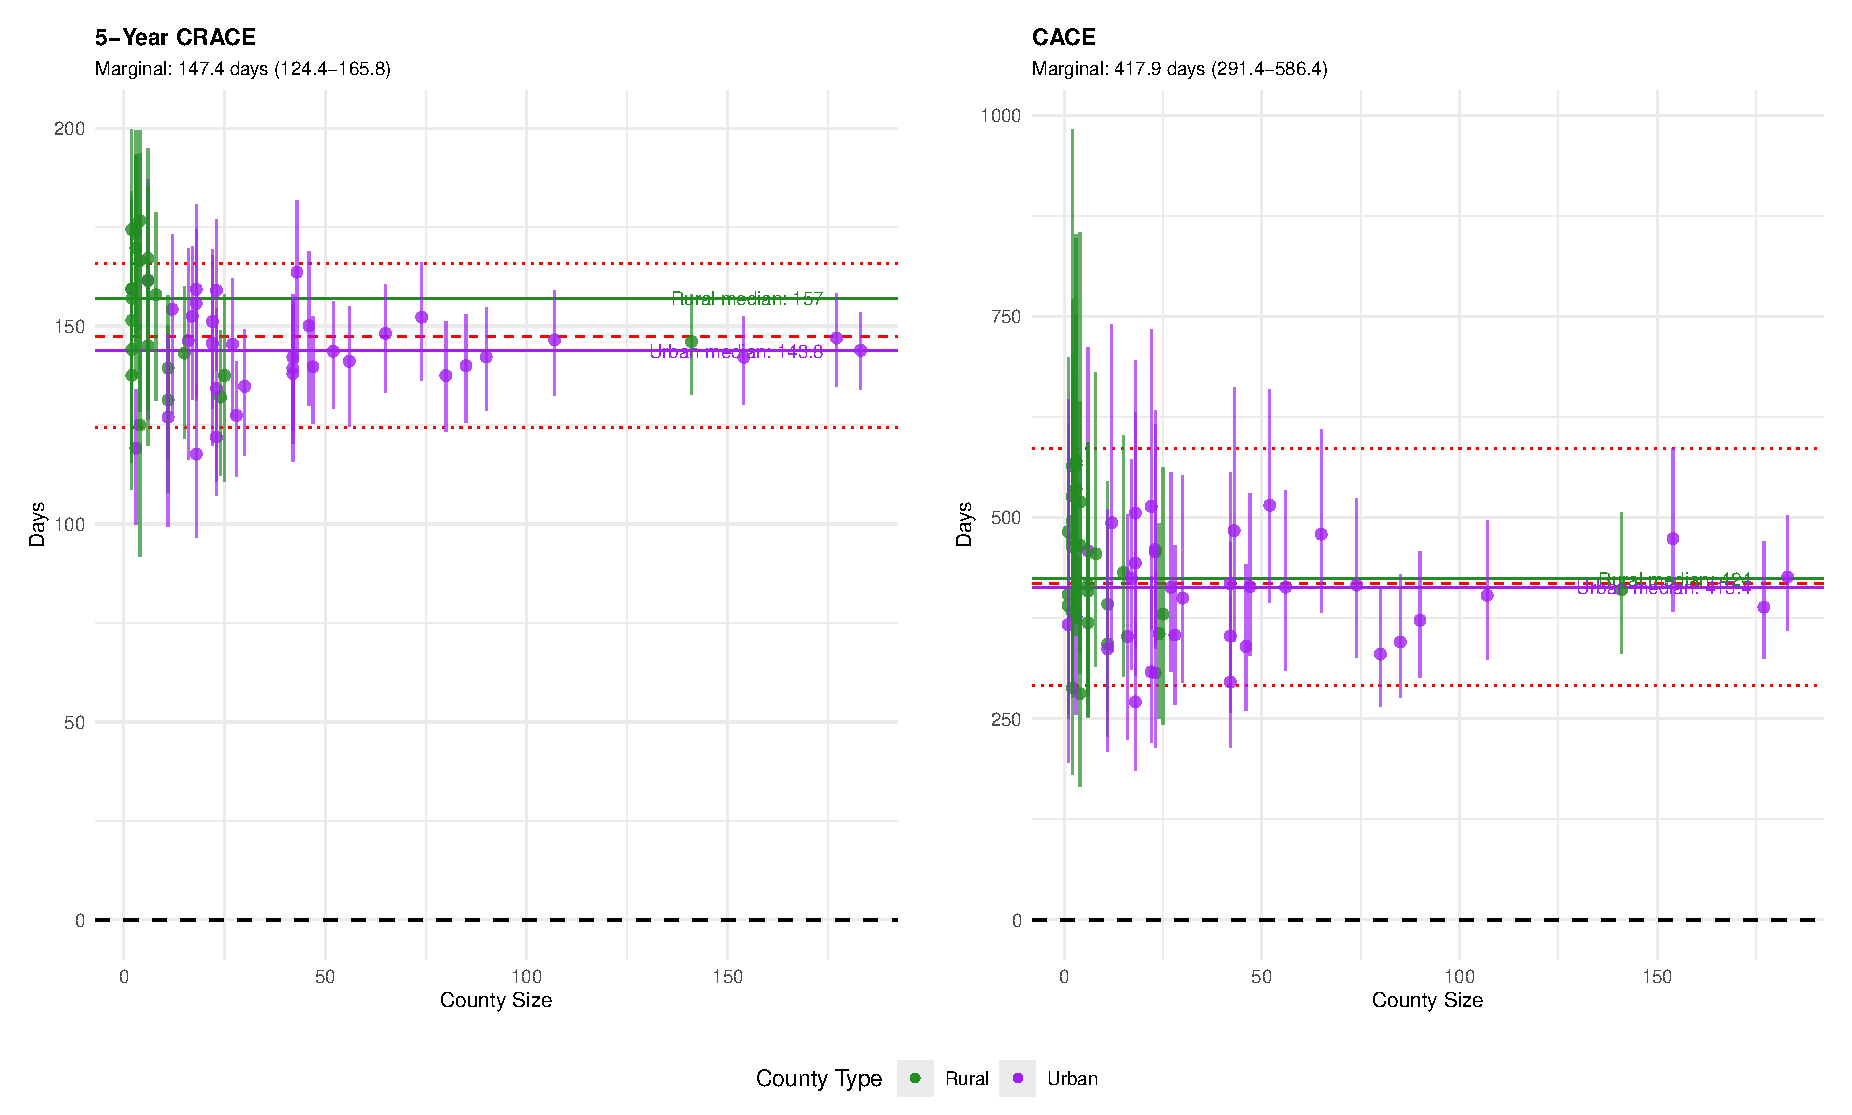
\includegraphics[width=\textwidth]{pics/CRACE_RACE_VS_SIZE.pdf}
  
  \end{frame}

 

  \begin{frame}{}
    \begin{columns}
  
        \column{0.6\textwidth}
    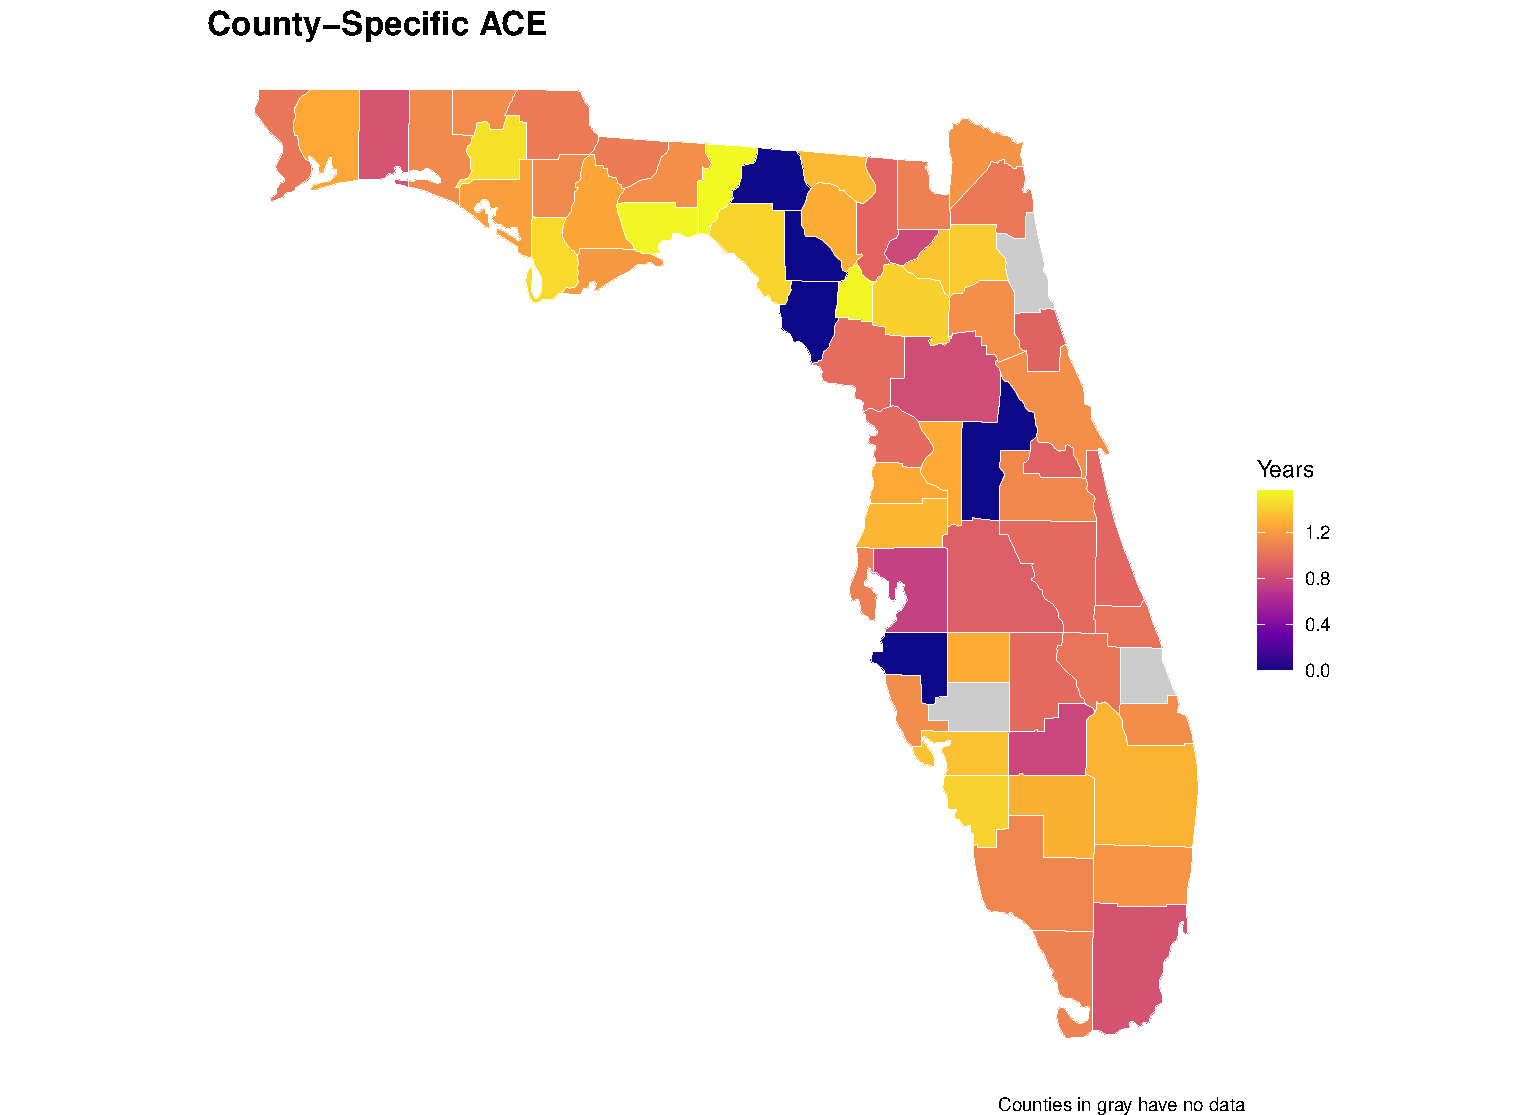
\includegraphics[width=1.1\textwidth]{pics/MapCACE.pdf}
    \column{0.38\textwidth}
    \begin{block}{Geographic Distribution}
        \begin{itemize}
        \item Northern regions: highest effects ($>$1.0 year)
        \item Central Florida: moderate effects ($\sim$0.8 years)
        \item Scattered counties: minimal effects ($<$0.3 years)
       % \item Eastern coastal counties: moderate-to-strong effects
        \item Spatial clustering suggests regional healthcare factors
        \end{itemize}
        \end{block}
    \end{columns}
  \end{frame}

  \begin{frame}{}
    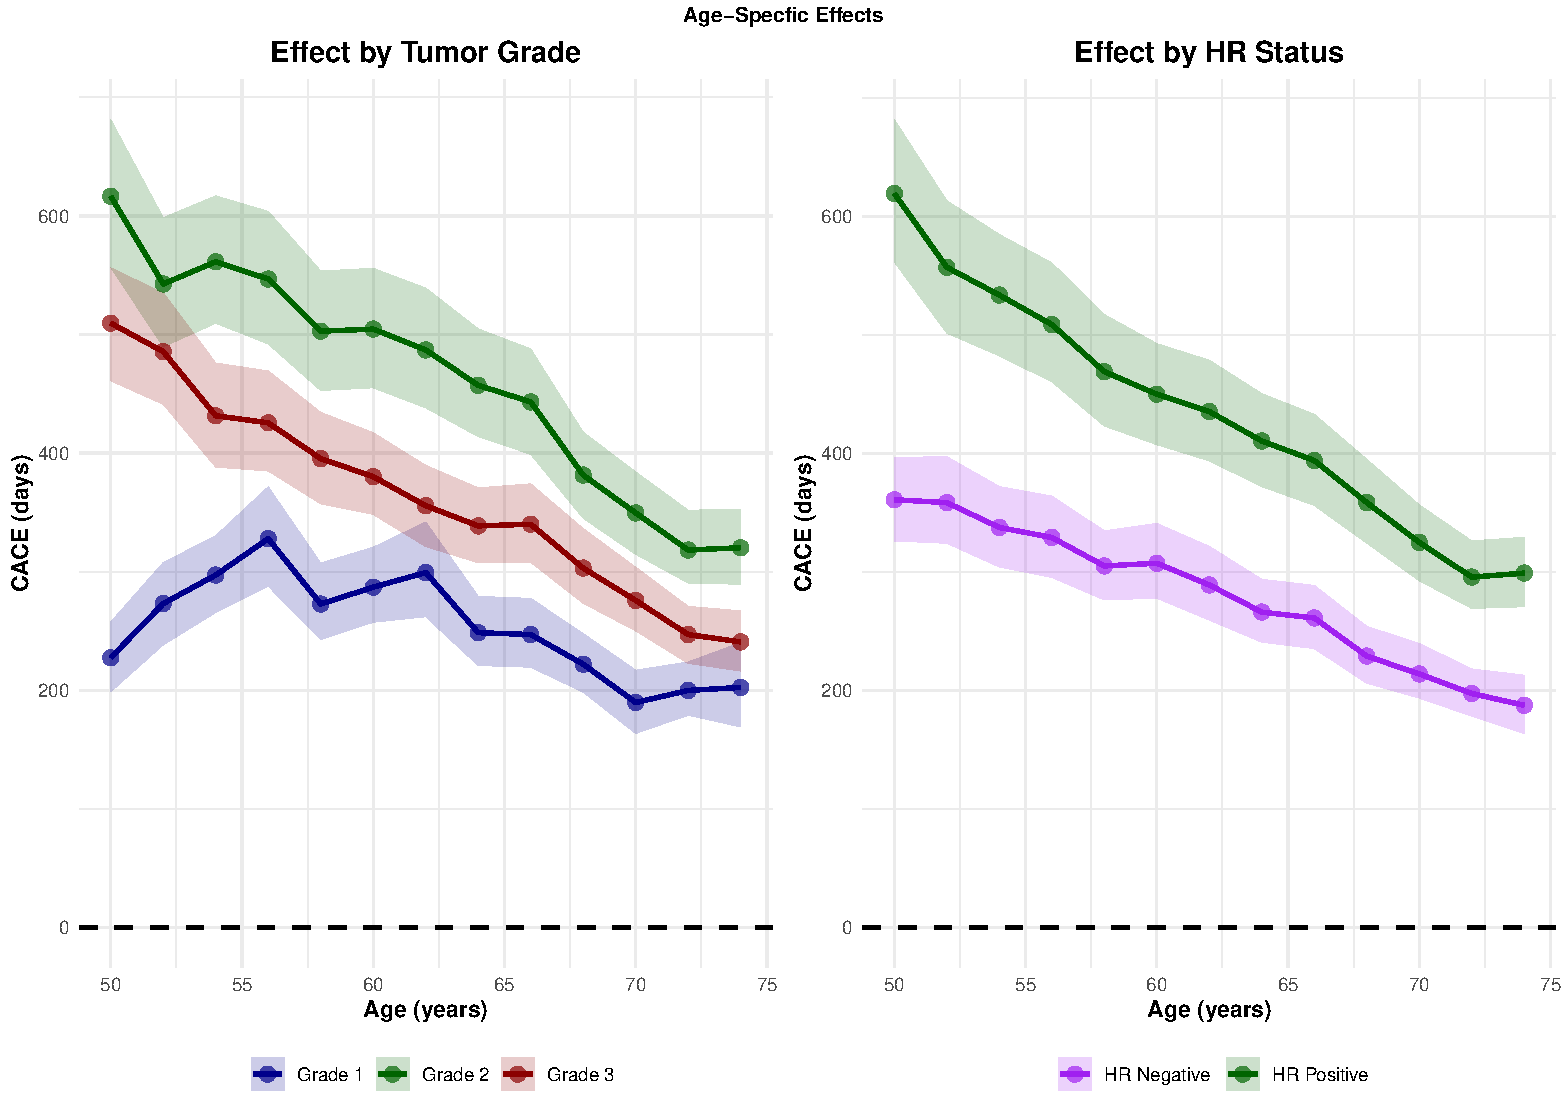
\includegraphics[width=\textwidth]{pics/Age_Specific Effects.pdf}
  
  \end{frame}
% Slide 1

    % Slide 2
    \begin{frame}{}
    
   
    
    \begin{block}{Age Effects (50-75 years)}
    \begin{itemize}
    \item Consistent decline in benefit with increasing age
    %\item Maximum benefit at age 50 ($\sim$620 days for Grade 2/HR+)
   % \item Minimum benefit at age 75 ($\sim$180 days for HR-)
   % \item Younger patients: prioritize to avoid delays
   % \item Even oldest patients maintain positive benefit
    \end{itemize}
    \end{block}
    
    \begin{block}{Tumor Characteristics}
    \begin{itemize}
    \item Grade 2: highest benefit (620$\rightarrow$320 days)
    \item Grade 3: moderate benefit (500$\rightarrow$250 days)
    \item Grade 1: lowest benefit (230$\rightarrow$200 days)
    \item HR+ status: substantially higher benefit (620$\rightarrow$300 days)
    \item HR- status: lower benefit (360$\rightarrow$180 days)
   \item HR status more impactful than tumor grade
    \end{itemize}
    \end{block}
    
    \begin{block}{Clinical Implications}
    \begin{itemize}
    \item Highest priority: young, HR+, Grade 2 patients ($>$600 days benefit)
    \item Lowest priority but still beneficial: older, HR-, Grade 1 patients ($\sim$180 days)
    \item Rural settings: ensure timely access despite geographic barriers
    \item Benefit persists beyond 5 years for most patients
    \item All patient subgroups gain survival advantage from avoiding delays
    \end{itemize}
    \end{block}
    
   
    \end{frame}
    \begin{frame}{Insights}
    
    
      \small
          
          \begin{block}{County-Level Effects}
          \begin{itemize}
          \item Average survival benefit: 417.9 days (95\% CI: 291.4--586.4)
          \item 5-year restricted benefit (CRATE): 147.4 days (95\% CI: 124.4--165.8)
          \item All counties show positive effects regardless of size
          \item Rural counties: slightly higher benefit (median 424 vs 413.4 days)
          \item No correlation between county size and effect magnitude
          \end{itemize}
          \end{block}
          
         
          
          \begin{block}{Consistency of Benefits}
          \begin{itemize}
          \item CRATE estimates more precise than CATE (narrower CIs)
          \item Universal positive effect: all counties above zero
          \item 5-year CRATE shows lasting impact of early treatment
          \end{itemize}
          \end{block}
          
      
          \end{frame}
          

    \begin{frame}{Conclusions}
        \begin{itemize}
          \vfill \item \textbf{Methodological Contributions:}
          \begin{itemize}
            \vfill \item First framework integrating causal inference with spatial survival data
            \vfill \item SoftBART with CAR priors for complex treatment-outcome relationships
            \vfill \item Doubly robust estimation for clustered survival outcomes
          \end{itemize}
          \vspace{6pt}
          \vfill \item \textbf{Key Findings:}
          \begin{itemize}
            \vfill \item 418-day survival benefit from avoiding treatment delays
            \vfill \item Universal positive effects across all counties
            \vfill \item Strongest benefits: younger, HR+, Grade 2 patients
          \end{itemize}
          \vspace{6pt}
          \vfill \item \textbf{Clinical Implications:}
          \begin{itemize}
            \vfill \item Prioritize timely treatment, especially in high-benefit groups
            \vfill \item Address regional healthcare disparities
          \end{itemize}
          \vspace{6pt}
          \vfill \item \textbf{Future Work:}
          \begin{itemize}
            \vfill \item Handle missingness in county data 
            \vfill \item Extend to other healthcare settings and outcomes
          \end{itemize}
        \end{itemize}
        \end{frame}
\begin{frame}
\frametitle{Thank You}
\begin{center}
Questions?
\end{center}
\end{frame}



\section{More Details on Computation}


\begin{frame}{Observed Data Likelihood}
  \begin{itemize}
    \item For each subject \(j\) in cluster \(i\), we observe
      \[
      y_{ij} = \min(T_{ij}, C_{ij}), \quad \delta_{ij} = \mathbbm{1}(T_{ij} < C_{ij}).
      \]
    \item Define the model mean (on the log-scale) as
      \[
      \mu_{ij} = f(z_{ij}, \mathbf{x}_{ij}, \mathbf{v}_i, \hat{e}(\mathbf{x}_{ij},\mathbf{v}_i)) + W_i.
      \]
      L_{ij}^{\text{obs}}(\theta) = \left\{ \frac{1}{\sqrt{2\pi\sigma^2}}
      \exp\!\left[-\frac{(\log y_{ij} - \mu_{ij})^2}{2\sigma^2}\right] \right\}^{\delta_{ij}}
      \left\{ 1 - \Phi\!\left(\frac{\log y_{ij} - \mu_{ij}}{\sigma}\right) \right\}^{1-\delta_{ij}},
      \]
      where \(\Phi(\cdot)\) is the standard normal CDF.
    \item The full observed-data likelihood is
      \[
      L_{\text{obs}}(\theta) = \prod_{i=1}^K \prod_{j=1}^{n_i} L_{ij}^{\text{obs}}(\theta).
      \]
  \end{itemize}
\end{frame}

\begin{frame}{ Data Augmentation}
  \begin{itemize}
    %\item \textbf{Priors:} Regularizing priors are assigned to the BART tree structures \(\{\mathcal{T}_h\}\) and terminal node parameters \(\{\mu_{lh}\}\).
    \item  Define the latent log survival time \( \tilde{y}_{ij}\) as
      \[
      \tilde{y}_{ij} =
      \begin{cases}
        \operatorname{TruncNormal}\Bigl(\mu_{ij},\sigma^2;\log y_{ij}\Bigr), & \text{if } \delta_{ij}=0, \\[1ex]
        \log y_{ij}, & \text{if } \delta_{ij}=1.
      \end{cases}
      \]
      Here, \(\operatorname{TruncNormal}(\mu,\sigma^2;a)\) denotes a \(N(\mu,\sigma^2)\) distribution truncated to the interval \((a,\infty)\). The imputed values are used in the complete-data likelihood.
  \end{itemize}
\end{frame}

\begin{frame}{Complete Data Likelihood}
  \begin{itemize}
    \item Introduce the latent (complete) log survival times:
      \[
      \tilde{y}_{ij} =
      \begin{cases}
        \log y_{ij}, & \delta_{ij}=1, \\[1ex]
        \text{draw from } N(\mu_{ij},\sigma^2) \text{ truncated to } [\log y_{ij},\infty), & \delta_{ij}=0.
      \end{cases}
      \]
    \item With \(\mu_{ij}\) defined as before, the complete-data likelihood is
      \[
      L_{\text{complete}}(\theta) = \prod_{i=1}^K \prod_{j=1}^{n_i} \frac{1}{\sqrt{2\pi\sigma^2}}
      \exp\!\left[-\frac{(\tilde{y}_{ij} - \mu_{ij})^2}{2\sigma^2}\right].
      \]
  \end{itemize}
\end{frame}


% Slide: Algorithm 1: A Single Iteration
\begin{frame}{Algorithm 1: A Single Iteration}
  \begin{enumerate}
    \item \textbf{Update Spatial Random Effects \& Variance:} Update \(W\), \(\tau^2\), and \(\rho\) from their full conditionals based on the CAR prior.
    
    \item \textbf{Impute Censored Data:} For subjects $ij$, sample the latent log survival time as
      \[
      \tilde{y}_{ij} =
      \begin{cases}
        \operatorname{TruncNormal}\Bigl(\mu_{ij},\sigma^2;\log y_{ij}\Bigr), & \text{if } \Delta_{ij}=0, \\[1ex]
        \log y_{ij}, & \text{if } \Delta_{ij}=1.
      \end{cases}
      \]
    \item \textbf{Update BART:} With responses \(\tilde{y}_{ij} - W_i\) and covariates \((z_{ij},\mathbf{x}_{ij})\), update the BART parameters \(\{\mathcal{T}_h,\mathcal{M}_h\}\) and the error variance \(\sigma^2\) via Bayesian backfitting.
    
  \end{enumerate}
\end{frame}





 

\end{document}